\chapter{Meritve}
Simulacije so prikazale okvirne poteke $sin$ in $cos$ signalov ter napake  ob posameznih ekscentričnostih.
Na merilni napravi so bile opravljene meritve ekscentričnosti. V poglavju je opisana merilna naprava, zajem podatkov ter izvedba meritev.
\section{Oprema in postavitev merilnega mesta}
Merilno mesto sestavljala krmilna plošča za regulacijo motorskega pogona in obdelavo signalov sestavljena v LRTME.
Vsebuje elektromotorski pogon z inkrementalnim, referenčnim dajalnikom zasuka TONiC podjetja Renishaw in magnetnim aktuatorjem za RM44 podjetja RLS  d.o.o.
Magnetni aktuator je možno premikati le v eni prostorski osi (slika \ref{premikanjeMagneta}).
Senzor RM44 je pritrjen na konstrukcijo 6-osnega mikrometrskega nastavljalnika pozicije HTIMS601.
Celotno merilno mesto je prikazano na sliki \ref{postavitevmerilnegamesta.jpg}.
\begin{figure}[h]
	\centering
	\includegraphics[width=0.4\columnwidth]{./Slike/premikanjeMagneta.jpg}
	\caption{Dinamično ekscentričnost se lahko izmeri le v eni smeri}
	\label{premikanjeMagneta}
\end{figure}
\begin{figure}[h!]
	\centering
	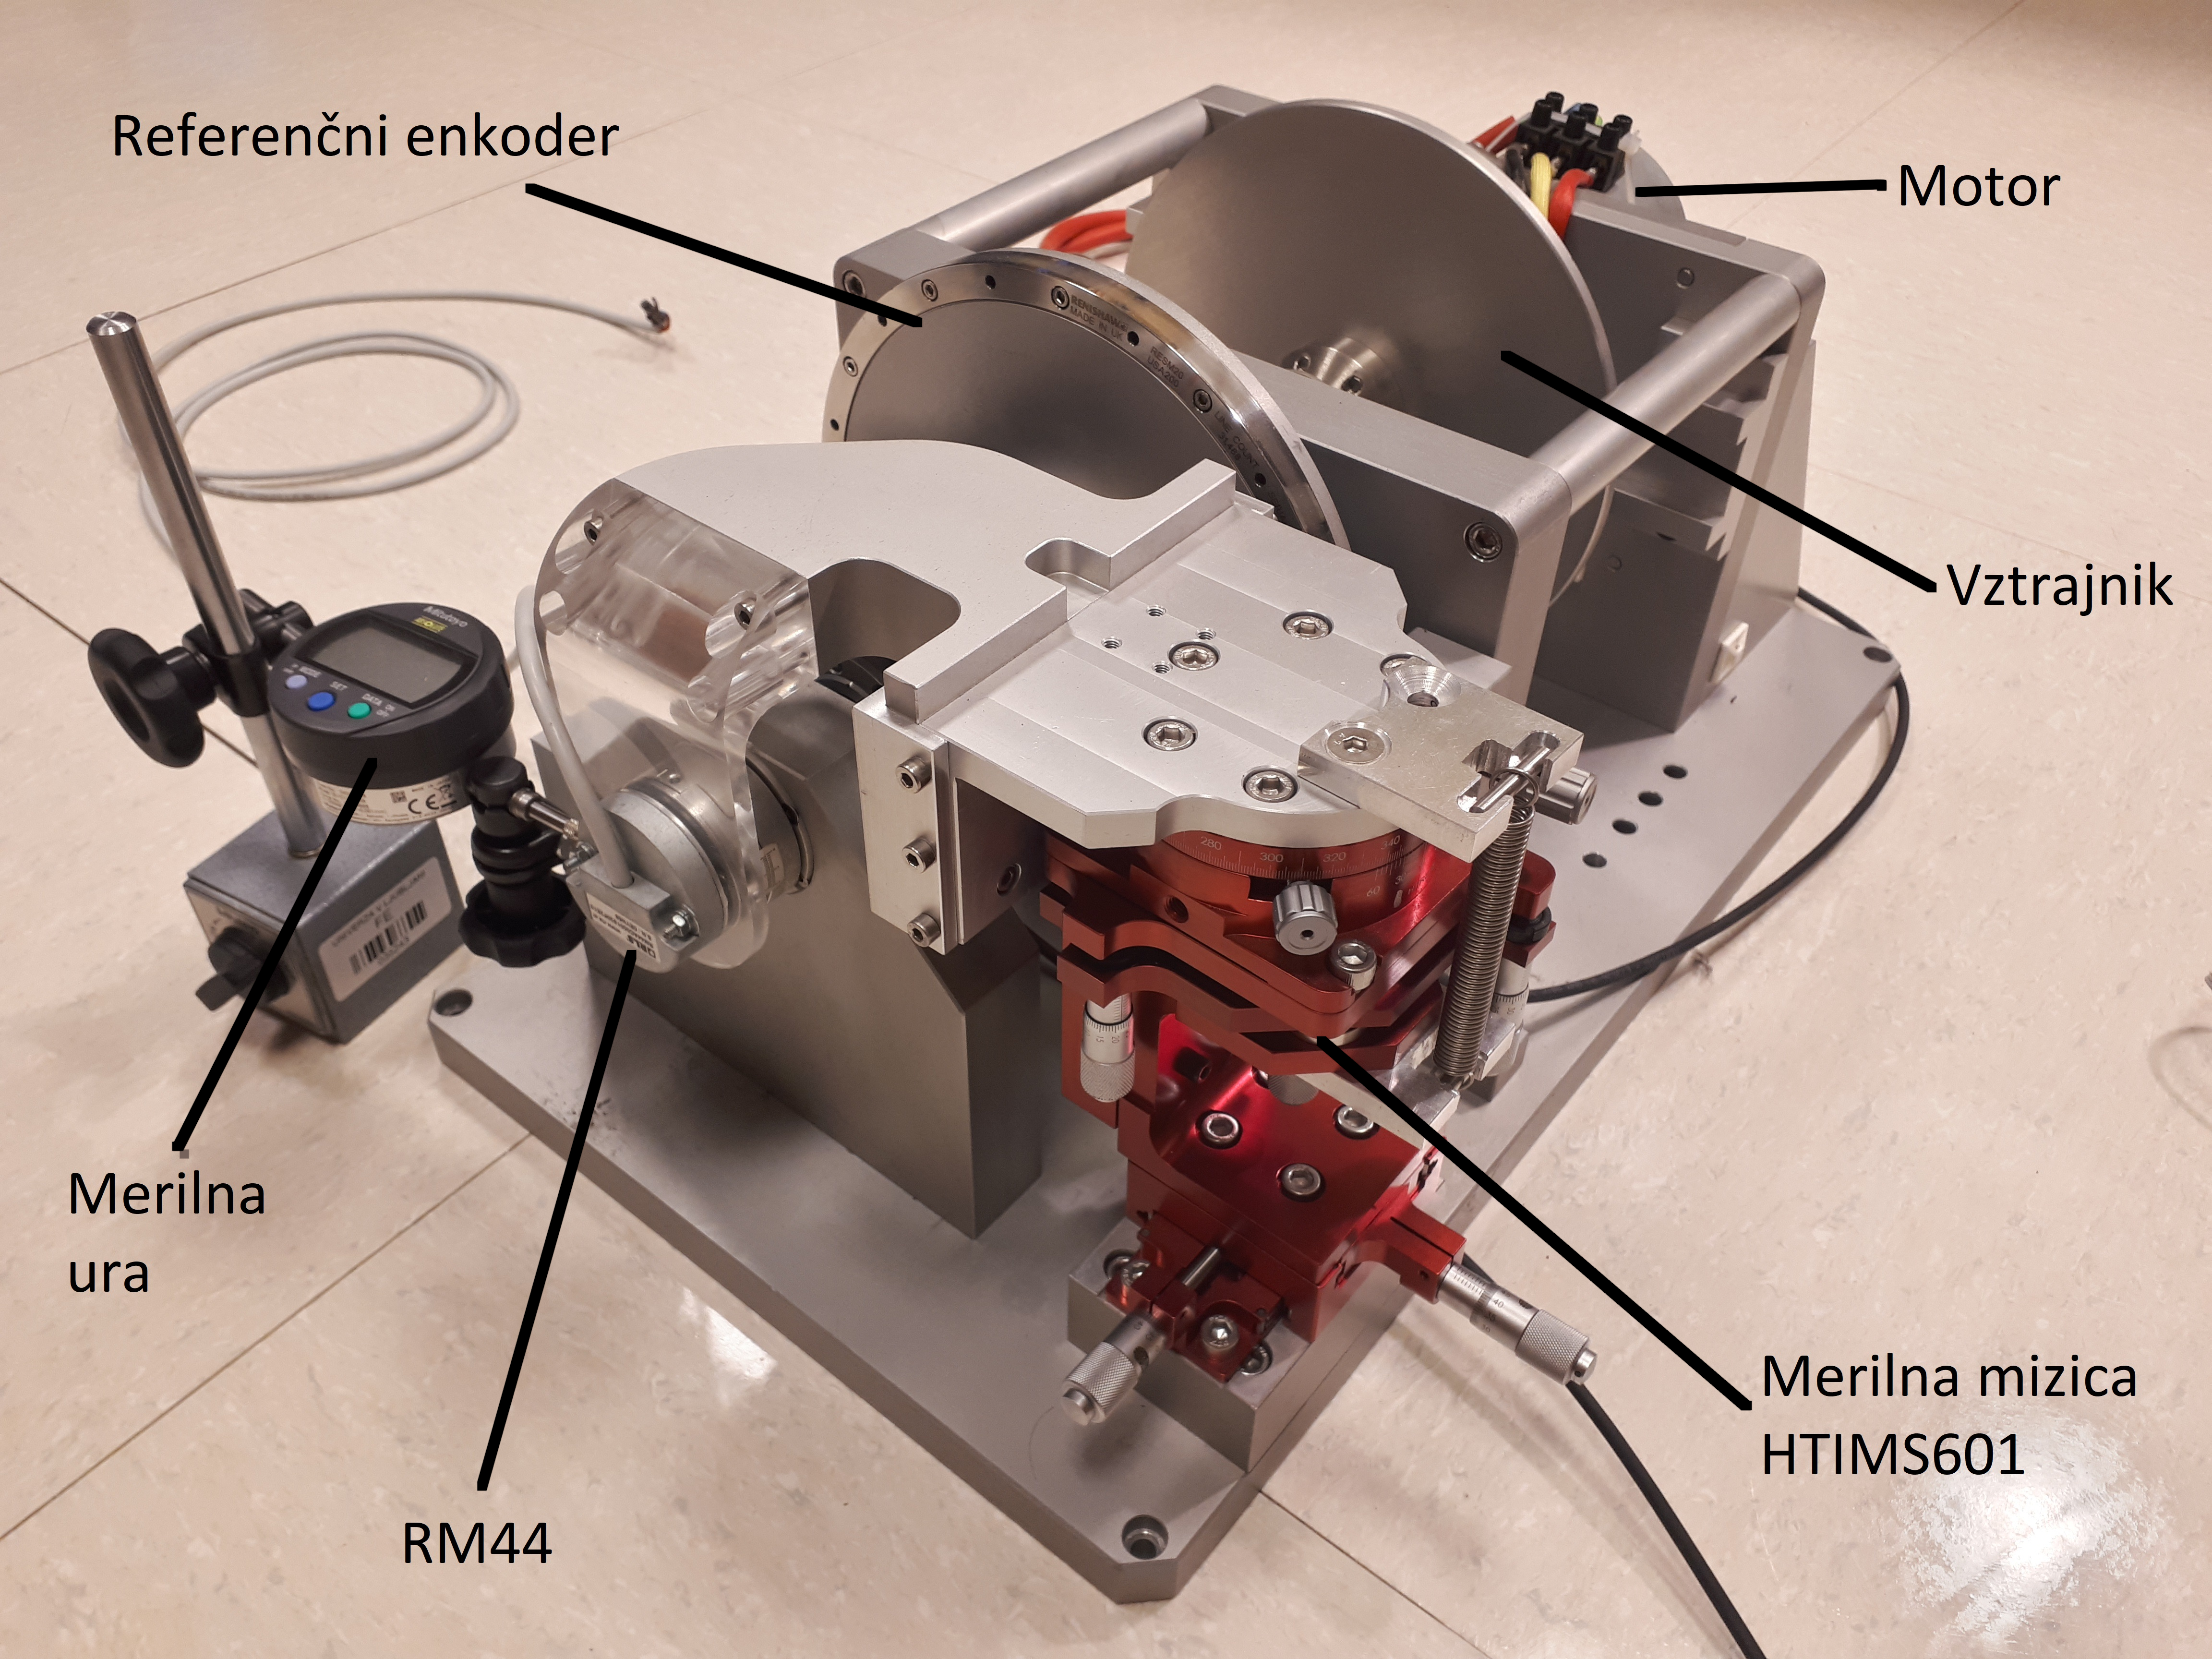
\includegraphics[width=0.75\textwidth]{./Slike/postavitevmerilnegamesta.jpg}
	\caption{Postavitev testnega mesta}
	\label{postavitevmerilnegamesta.jpg}
\end{figure}
\begin{figure}[h!]
	\centering
	\includegraphics[width=0.65\textwidth]{./Slike/koordinatnisistem.jpg}
	\caption{Postavitev testnega mesta}
	\label{koordinatnisistem.jpg}
\end{figure}
\begin{figure}[h!]
	\centering
	\includegraphics[width=0.55\textwidth]{./Slike/HTIMS601.jpg}
	\caption{Naprava za nastavljanje statične ekscentričnosti}
	\label{HTIMS601.jpg}
\end{figure}
Za manevriranje s HTIMS601 je potrebno nastaviti 6 osi.
S postavitvijo koordinatnega sistema (slika \ref{koordinatnisistem.jpg}), je vsak od vijakov definiral premik senzorja. 
Vsako os se nastavlja z enim od vijakov (slika \ref{HTIMS601.jpg}). Vijaki poimenovani x-os, y-os in z-os so za nastavljanje translaciijo merjenca, x-rot, y-rot in z-rot so za nastavljanje rotacije premikajoče plošče na vrhu HTIMS601.
S spremembo vrtenja vijakov translacijskih osi, se je lokacija senzorja pred magnetom spreminjala za enako spremembo. S spremembo vrtenja rotacijskih vijakov, se je zaradi ročice na katero je pritrjen senzor, senzor zarotira in hkrati tudi premakne iz dotedanje lege. S spremembo rotacije je potrebno popraviti tudi nastavitve vijakov, ki senzor premikajo v translacijskih oseh.

Hitrost vrtenja pogona je nastavljiva.
Hitrost vrtenja je pogona je nastavljena na 60 RPM. Hitrost ni popolnoma konstantna (slika \ref{hitrost}). Vzrok je v vztrajnosti pogona. Mitja Nemec je problem skušal čimbolje odpraviti, z dodajanjem primernih uteži na primerna mesta na vztrajniku.
\slikaeps{Potek hitrosti od zasuka}{hitrost}
\newpage
\section{Zajem podatkov}
Mitja Nemec je pripravil grafični uporabniški vmesnik za prikazovanje meritev (slika \ref{GUI.png}).
Vmesnik lahko prikazuje potek refernečnega kota, $sin$ in $cos$ senzorja RM44, izračunanega kota iz $sin$ in $cos$ signala, napako med izračunanim kotom senzorja in refernčnim dajalnikom, hitrost vrtenja ter tok prve faze motorskega pogona. Signaloma $sin$ in $cos$ se v programu prišteje enosmerna komponenta, ki bi popravila izhodna signala.

Krmilna plošča (slika \ref{krmilnaplosca.jpg}) zajema podatke s pogona s frekvenco 1kHz.
Referenčni inkrementalni dajalnik, se ob zagonu inicializira. V programu se podatek o kotu deli z 12595200. Definicijsko območje referenčnega kota se giblje med 0 in 1.
Signala sin in cos se na krmilni plošči ojačata in pretvorita z 12 bitnim AD pretvornikom. Izhodu AD pretvornika se odšteje 2048 in deli s 4096. Definicijsko območje sin in cos signala se gibljeta med $\pm0,5$.
Hitrost in napaka sta izračunana iz zajetih signalov.
Podatki so v obliki enega paketa poslani s krmilne plošče na 1 sekundo. Pri frekvenci vrtenja 1 Hz, grafični vmesnik prikaže en obrat.
Podatke se lahko izvozi v obliki .csv datoteke in nato poljubno obdela.
Na sliki  \ref{GUI.png} je prikazan sinusni signal prikazan kot da je zamaknjen za 180$\mathrm{^\circ}$. To je posledica definicije pozitvne smeri vrtenja za senzor \cite{RM44}. Senzor ima nasproto definirano pozitivno smer vrtenja. To sem rešil tako, da sem obrnil podatke. Popraviti je bilo potrebno tudi potek referenčnega dajalnika.
\bitnaslika{Grafični vmesnik s poteki signalov}{GUI.png}{0.8\textwidth}{0.42\textwidth}
\begin{figure}[h!]
	\centering
	\includegraphics[width=0.55\textwidth]{./Slike/krmilnaplosca.jpg}
	\caption{Krmilna plošča za krmiljenje pogona in obdelavo signalov s dajalnikov položaja}
	\label{krmilnaplosca.jpg}
\end{figure}
\newpage
\section{Senzor v izhodiščni legi}
Senzor in magnet se lahko gibljeta, najprimernejša, izhodiščna lega, ni definirana. Z merilno urico Mitutoyo 543-391B se je dinamično ekscentričnost magneta nastavilo na najmanjšo. Oplet z merilno urico je bil pomerjen $\pm 3 \mathrm{\mu m_{pp}}$.
S prilagajanjem vijakov HTIMS601, opazovanjem $sin$ in $cos$ ter napake je bil senzor nastavljen v lego, kjer je bila amplituda drugega harmonika napake najmanjša. Najprimernejšo lego sem iskal glede na vrednost amplitud in ortogonalnost  $sin$ in $cos$. Signala $sin$ in $cos$ morata ustrezati definicijskem območju zajema AD pretvornika.

Na sliki \ref{./MER/00_sincos} sta prikazana $sin$ in $cos$. Enosmerni komponenti sta prisotni v obeh signalih, posledično se izrazi v napaki prvi harmonik (slika \ref{./MER/00_napaka}).
V napaki se pojavi med $\mathrm{95^\circ}$ in $\mathrm{140^\circ}$ preskok napake. V signalih $sin$ in $cos$ se v tem območju pojavi fazni zamik, $sin$ pri $\mathrm{95^\circ}$ in nato $cos$ pri $\mathrm{160^\circ}$. Vzroka nisem raziskoval.
Z razvojem napake v Fourierovo vrsto (slika \ref{./MER/00_fft}) vidimo velikosti posameznih amplitud napake.
Enosmerna komponenta je posledica sofaznih zamikov obeh signalov $sin$ in $cos$. 
Prvi harmonik je posledica ensmermih komponent $sin$ in $cos$. Z matematično obdelavo siganlov $sin$ in $cos$ sem enosmerni komponenti odstranil,vendar se prvi harmonik napake še vedno izrazi. Prvi harmonik napake je odvisen tudi od drugega harmonika v signalih $sin$ in $cos$.
Z odstranitvijo tudi drugega harmonika iz signalov $sin$ in $cos$ je bil  prvi harmonik v napaki odstranjen.
Signala  $sin$ in $cos$ med izvajanjem meritev ne bosta spremenjena zaradi matematične obdelave. Spreminjanje signalov  $sin$ in $cos$ in napake se bo opazovalo glede na potek, ki je bil pomerjen v izhodiščni legi.
\slikaeps{Signala $sin$ in $cos$ pomerjena v izhodiščni legi}{./MER/00_sincos}
\slikaeps{Napaka $\varepsilon$ pomerjena v izhodiščni legi}{./MER/00_napaka}
\slikaeps{Amplitude harmonikov napake $\varepsilon$ razvite v Fourierovo vrsto pri meritvah v izhodiščni legi}{./MER/00_fft}
\newpage
\subsection{Meritve v izhodišni legi}
V izhodiščni legi je bilo opravljenih več meritev. Osredotočil sem se na enosmerni komponenti  in amplitudi osnovnega harmonika $sin$ in $cos$. 
Porazdelitev enosmerne komponente signala $sin$ in $cos$ je prikazana na sliki \ref{./MER/00_off}.
Srednja vrednost enosmerne komponente $sin$ je $-8,85 \cdot 10^{-4}$, standardna deviacija je $1,08\cdot 10^{-4}$.
Srednja vrednost enosmerne komponente $cos$ je $4,20 \cdot 10^{-3}$, standardna deviacija je $5,20\cdot 10^{-5}$.
\slikaeps{Porazdelitev meritev enosmerne komponente signalov $sin$ in $cos$}{./MER/00_off}
Porazdelitev amplitude osnovnega harmonika signala $sin$ in $cos$ je prikazana na sliki \ref{./MER/00_off}.
Srednja vrednost amplitude osnovnega harmonika $sin$ je $0,451$, standardna deviacija je $2,20\cdot 10^{-4}$.
Srednja vrednost amplitude osnovnega harmonika $cos$ je $0,449$, standardna deviacija je $1,95\cdot 10^{-4}$.
\slikaeps{Porazdelitev meritev amplitude osnovnega harmonika signalov $sin$ in $cos$}{./MER/00_amp}
\newpage
\section{Meritve statične ekscentričnosti v smeri x-osi}
Pri meritvi je pričakovati spremembo amplitud in faznih zamikov signalov $sin$ in $cos$. Na sliki \ref{./MER/xs_sincos} sta prikazana $sin$ in $cos$ pomerjena pri 0,20 mm statične ekscentričnosti v smeri x. Na signalih, med 95 in 175$^\circ$ se pojavijo nenavadni skoki.
Izrazijo se tudi na napaki, ki je prikazana na sliki \ref{./MER/xs_napaka}. Med 95 in 175$^\circ$ se signala $sin$ in $cos$ hkrati fazno zamakneta. Vzrok tega pojava nisem raziskoval. Napaka razvita v Fourierovo vrsto prikaže pričakovano povišanje drugega harmonika. Povišala sta se tudi amplitudi tretjega in četrtega harmonika.
\slikaeps{Signala $sin$ in $cos$ merjena pri 0,2 mm statične ekscentičnosti v smeri x}{./MER/xs_sincos}
\slikaeps{Napaka $\varepsilon$ merjena pri 0,2 mm statične ekscentičnosti v smeri x}{./MER/xs_napaka}
\slikaeps{Amplitude harmonikov napake $\varepsilon$ razvite v Fourierovo vrsto merjeno pri 0,2 mm statične ekscentičnosti v smeri x}{./MER/xs_fft}
\newpage
\subsection{Sprememba $sin$, $cos$ ter napake od $\Delta x_s$}
Iz simulacij se pričakuje zmanjševanje amplitude osnovnega harmonika $cos$ signala- Sprememba amplitud osnovnih harmonikov je prikazana na sliki \ref{./MER/xs_sincos_amp}. Amplituda signala $cos$ pada pričakovano, pada tudi ampituda signala $sin$. Signala nimata enake amplitude v izhodišču, kar je posledica neidealne izhodiščne lege. Potek enosmerne komponente je prikazan na sliki \ref{./MER/xs_sincos_off}. Komopnenta $cos$ signala pada kot je bilo predvideno v simulacijah. Fazni zamik signalov je prikazan na sliki \ref{./MER/xs_sincos_phase}. Pričakovano po simulacijah se fazna razlika med signaloma zmanjšuje. Rezultati simulacij so prikazovali konstanten fazni kot signala $cos$ in spreminjanje le faznega kota $sin$. Pri meritvah se je fazni kot $cos$ zmanjševal, fazni kot $sin$ naraščal. Razlika med njima je manjša, kot je bila posimulirana. Vsota faznih zamikov ostaja konstantna, zato se enosmerna komponenta v napaki ne spreminja.
Poteki posameznih komponent signalov $sin$ in $cos$ so aproksimirani s kubičnimi polinomi.
\slikaeps{Potek amplitude osnovnega harmonika $sin$ in $cos$ pri meritvah statične ekscentričnosti v smeri x}{./MER/xs_sincos_amp}
\slikaeps{Potek enosmerne komponente $sin$ in $cos$ pri meritvah statične ekscentričnosti v smeri x}{./MER/xs_sincos_off}
\slikaeps{Fazni zamik osnovnega harmonika  $sin$ in $cos$ pri meritvah statične ekscentričnosti v smeri x  glede na idealna signala $sin$ in $cos$}{./MER/xs_sincos_phase}
\begin{eqnarray}
&A_{sin} = -6,14\cdot 10^{-2}\Delta x_s^3-1,71\cdot 10^{-2}\Delta x_s^2-1,17\cdot 10^{-2}\Delta x_s+0,484\\  
&Off_{sin} = -0,0388\Delta x_s^3+0,0237\Delta x_s^2-2,25\cdot 10^{-3}\Delta x_s-9,53\cdot 10^{-4}            \\
&\delta_{sin} = 5,32 \Delta x_s^3-3,55\Delta x_s^2+3,49\Delta x_s+1,08           \\ 
&A_{cos} = 7,46\cdot 10^{-3}\Delta x_s^3-0,185\Delta x_s^2+1,01\cdot 10^{-2}\Delta x_s+0,488\\  
&Off_{cos} = 0,0221\Delta x_s^3-0,191\Delta x_s^2-3,91\cdot 10^{-3}\Delta x_s+6,48\cdot 10^{-3}            \\
&\delta_{cos} = 11,5  \Delta x_s^3-10,6\Delta x_s^2-1,14\Delta x_s+1,19
\end{eqnarray}

Slika \ref{./MER/xs_potek} prikazuje poteke amplitud posameznih harmonikov napake v odvisnosti od statične ekscentričnosti v smeri x. Kvadratično narašča amplituda drugega harmonika, medtem ko so enosmerna komponenta in ostali harmoniki konstantni. Poteke se aproksimira s kubičnimi polinomi.
\slikaeps{Potek amplitud posameznega harmonika napake $\varepsilon$ pri meritvah statične ekscentričnosti v smeri x}{./MER/xs_potek}
\begin{eqnarray}
&C_0 =2,42\Delta x_s^{3}-1,71\Delta x_s^{2}+2,40\cdot 10^{-1}\Delta x_s+1,15 \\              
&C_1 =-3,01\Delta x_s^{3}+2,35\Delta x_s^{2}-6,35\cdot 10^{-1}\Delta x_s+1,21 \\             
&C_2 =-1,11\Delta x_s^{3}+5,06\Delta x_s^{2}+9,95\cdot 10^{-1}\Delta x_s+1,18\cdot 10^{-1} \\
&C_3 =-2,10\Delta x_s^{3}+1,61\Delta x_s^{2}-5,25\cdot 10^{-1}\Delta x_s+3,57\cdot 10^{-1} \\
&C_4 =-3,24\Delta x_s^{3}+2,29\Delta x_s^{2}-4,73\cdot 10^{-1}\Delta x_s+4,17\cdot 10^{-1}
\end{eqnarray}
\section{Meritve statične ekscentričnosti v smeri y-osi}
Slika \ref{./MER/ys_sincos} prikazuje zajeta signala $sin$ in $cos$ pri statični ekscentričnosti v smeri y. Amplituda $sin$ se je zmanjšala, kot je bilo pričakovati po rezultatih simulacij. Posledično se izrazi v napaki višji drugi harmonik (slika \ref{./MER/ys_napaka}). Z razvojem napake v Fourierovo vrsto se potrdi povišanje drugega harmonika.Enosmerna komponenta in prvi harmonik sta nekoliko nižja.
\slikaeps{Signala $sin$ in $cos$ merjena pri 0,2 mm statične ekscentičnosti v smeri y}{./MER/ys_sincos}
\slikaeps{Napaka $\varepsilon$ merjena pri 0,2 mm statične ekscentičnosti v smeri y}{./MER/ys_napaka}
\slikaeps{Amplitude harmonikov napake $\varepsilon$ razvite v Fourierovo vrsto merjeno pri 0,2 mm statične ekscentičnosti v smeri y}{./MER/ys_fft}
\newpage
\subsection{Sprememba $sin$, $cos$ ter napake od $\Delta y_s$}
Slika \ref{./MER/ys_sincos_amp} prikazuje potek amplitud osnovnega hamonika napake v odvisnosti statične ekscentričnosti v smeri y. S potekov se opazi padanje amplitud. Razlika med signaloma linearno narašča. 
Slika \ref{./MER/ys_sincos_off} prikazuje potek enosmernih komponent. Pri meritvi 0,15 mm se pojavi skok enosmernih komponent, vendar razlika ostaja enaka.
Fazni kot se v pri manjših odmikih ne spreminja kot je bilo pričakovati po rezultatih simulacij. Pri večjih odmikih se sprememba faznih kotov izrazi kot se je pričakovalo. Fazna razlika se začne ob večjih izmikih manjšati.
\slikaeps{Potek amplitude osnovnega harmonika $sin$ in $cos$ pri meritvah statične ekscentričnosti v smeri y}{./MER/ys_sincos_amp}
\slikaeps{Potek enosmerne komponente $sin$ in $cos$ pri meritvah statične ekscentričnosti v smeri y}{./MER/ys_sincos_off}
\slikaeps{Fazni zamik osnovnega harmonika  $sin$ in $cos$ pri meritvah statične ekscentričnosti v smeri y glede na izhodiščno lego}{./MER/ys_sincos_phase}
\begin{eqnarray}
&A_{sin} = 1,73            \Delta y_s^3-6,47\cdot 10^{-1}\Delta y_s^2-2,60\cdot 10^{-1}\Delta y_s+4,94\cdot 10^{-1}            \\    
&Off_{sin} = +0,0469\Delta y_s^3+0,0132\\Delta y_s^2-0,0229\Delta y_s+7,08\cdot 10^{-4}            \\ 
&\delta_{sin} = +3,37\cdot 10    \Delta y_s^3-2,12\cdot 10^{1}\Delta y_s^2+3,81            \Delta y_s^1+8,82\cdot 10^{-1}            \\ 
&A_{cos} = +1,99            \Delta y_s^3-9,29\cdot 10^{-1}\Delta y_s^2-7,82\cdot 10^{-2}\Delta y_s+4,91\cdot 10^{-1}            \\    
&Off_{cos} = 0,187\Delta y_s^3-0,0792\Delta y_s^2-9,87\cdot 10^{-3}\Delta y_s+9,94\cdot 10^{-3}            \\ 
&\delta_{cos} = -1,76\cdot 10    \Delta y_s^3-9,77\cdot 10^{-1}\Delta y_s^2+4,42            \Delta y_s+3,59\cdot 10^{-1}
\end{eqnarray}

Slika \ref{./MER/ys_potek} prikazuje poteke amplitude posameznih harmonikov napake. Kot je bilo pričakovano se spreminja le amplituda drugega harmonika. 
\slikaeps{Potek amplitud posameznega harmonika napake $\varepsilon$ pri meritvah statične ekscentričnosti v smeri y}{./MER/ys_potek}
\begin{eqnarray}
&C_0 =-3,26\Delta y_s^{3}-3,10\Delta y_s^{2}+2,68\Delta y_s+6,00\cdot 10^{-1} \\                                      
&C_1 =-2,38\Delta y_s^{3}+3,50\Delta y_s^{2}-1,54\Delta y_s+1,12 \\                                                   
&C_2 =-4,15\Delta y_s^{3}-1,64\Delta y_s^{2}+8,22\Delta y_s+8,04\cdot 10^{-2} \\                                      
&C_3 =2,30\Delta y_s^{3}-1,37\cdot 10^{-1}\Delta y_s^{2}-3,13\cdot 10^{-1}\Delta y_s+1,78\cdot 10^{-1} \\             
&C_4 =7,11\cdot 10^{-1}\Delta y_s^{3}-7,96\cdot 10^{-2}\Delta y_s^{2}-3,14\cdot 10^{-1}\Delta y_s+3,21\cdot 10^{-1}
\end{eqnarray}
\section{Meritve dinamične ekscentričnosti v smeri x-osi}

Meritve dinamične ekscentričnosti so bile lahko pomerjene le v eni koordinatni osi. Os po kateri se na napravi spreminja ekscentričnost magneta je zasukana za 32,4$^\circ$ na abciso. Meritev zato ni bilo možno opraviti neposredno v eni koordinatni osi. Enačbe spodaj aproksimirajo poteke amplitude osnovnega harmonika, faze osnovnega harmonika in enosmerne komponete $sin$ in $cos$, ter poteke amplitud posameznega harmonika napke pri dinamični ekscentričnosti v smeri x in zarotiranem magnetu za 32,4$^\circ$ pri simulacijah z realnim magnetnim poljem. V enačbah je ekscentričnost označena z $\Delta x_{d}$, z zavedanjem, da je mišljen potek z zasukanim magnetom. 
\begin{eqnarray}
&A_{sin}=1,03\Delta x_d^3-5,83\cdot10^{0}\Delta x_d^2-3,77\cdot10^{-1}\Delta x_d+3,99\cdot10\\
&Off_{sin}=4,24\cdot10^{-1}\Delta x_d^3+6,40\cdot10^{-1}\Delta x_d^2-7,57\Delta x_d+1,29\cdot10^{-1}\\
&\delta_{sin}=-4,59\Delta x_d^3+7,50\cdot10^{0}\Delta x_d^2-4,12\cdot10^{-1}\Delta x_d-1,38\cdot10^{-1}\\
&A_{cos}=1,03\Delta x_d^3-5,83\cdot10^{0}\Delta x_d^2-3,77\cdot10^{-1}\Delta x_d+3,99\cdot10\\
&Off_{cos}=4,24\cdot10^{-1}\Delta x_d^3+6,40\cdot10^{-1}\Delta x_d^2-7,57\Delta x_d+1,29\cdot10^{-1}\\
&\delta_{cos}=-4,59\Delta x_d^3+7,50\cdot10^{0}\Delta x_d^2-4,12\cdot10^{-1}\Delta x_d-1,38\cdot10^{-1}
\end{eqnarray}
\begin{eqnarray}
&C_0 =-4,95\Delta x_d^{3}+6,52\Delta x_d^{2}-4,16\cdot 10^{-1}\Delta x_d-1,37\cdot 10^{-1} \\                         
&C_1 =-2,62\Delta x_d^{3}+2,78\Delta x_d^{2}+2,11\cdot 10\Delta x_d-2,89\cdot 10^{-2} \\                              
&C_2 =4,68\cdot 10^{-1}\Delta x_d^{3}+5,21\cdot 10^{-1}\Delta x_d^{2}-2,03\cdot 10^{-2}\Delta x_d+2,54\cdot 10^{-3} \\
&C_3 =-4,90\cdot 10^{-2}\Delta x_d^{3}+8,11\cdot 10^{-1}\Delta x_d^{2}+7,89\Delta x_d+1,25\cdot 10^{-1} \\            
&C_4 =1,04\cdot 10\Delta x_d^{3}-2,55\Delta x_d^{2}-2,82\cdot 10^{-1}\Delta x_d+2,96\cdot 10^{-1}
\end{eqnarray}
Poteki so podobni simulacijam brez zasukanega magneta, amplitude napake so nižje.

Pri dinamični ekscentričnosti v povzročeni smeri se signala $sin$ in $cos$ nista opazno spremenila (slika \ref{./MER/xd_sincos}). Sprememb ni niti na napaki (slika \ref{./MER/xd_napaka}). Spremembe niso opazne niti na  napaki razviti v Fourierovo vrsto (slika \ref{./MER/xd_fft}).
\slikaeps{Signala $sin$ in $cos$ merjena pri 0,19 mm dinamične ekscentičnosti v smeri x}{./MER/xd_sincos}
\slikaeps{Napaka $\varepsilon$ merjena pri 0,19 mm dinamične ekscentičnosti v smeri x}{./MER/xd_napaka}
\slikaeps{Amplitude harmonikov napake $\varepsilon$ razvite v Fourierovo vrsto merjeno pri 0,19 mm dinamične ekscentičnosti v smeri x}{./MER/xd_fft}
\subsection{Sprememba $sin$, $cos$ ter napake od $\Delta x_d$}

Potek spreminjanja amplitude osnovnega harmonika $sin$ in $cos$ glede na dinamično ekscentričnost pričakovano pada (Slika \ref{./MER/xd_sincos_amp}). Razlika med amplitudama ostaja tekom spreminjanja dinamične ekscentričnosti enaka. Enosmerni komponenti $sin$ in $cos$ padati, vendar vsaka s svojim gradientom. Sprememba enosmerne komponente je manjša, kot je bila predvidena v simulacijah. Sprememba faznega zamika osnovnega harmonika $sin$ in $cos$ je prikazana na sliki \ref{./MER/xd_sincos_phase}. Fazna zamika s spremebo dinamične ekscentričnosti naraščata. V simulacijah tako velika sprememba enosmerne komponente ni bila pričakovana.
\slikaeps{Potek amplitude osnovnega harmonika $sin$ in $cos$ pri meritvah dinamične ekscentričnosti v smeri x}{./MER/xd_sincos_amp}
\slikaeps{Potek enosmerne komponente $sin$ in $cos$ pri meritvah dinamične ekscentričnosti v smeri x}{./MER/xd_sincos_off}
\slikaeps{Fazni zamik osnovnega harmonika  $sin$ in $cos$ pri meritvah dinamične ekscentričnosti v smeri x glede na izhodiščno lego}{./MER/xd_sincos_phase}

Poteke prikazane na slikah \ref{./MER/xd_sincos_amp} \ref{./MER/xd_sincos_off} in \ref{./MER/xd_sincos_phase}, se lahko aproksimira s kubičnimi polinomi.
\begin{eqnarray}
&A_{sin}=-0,795\Delta x_d^3+0,405\Delta x_d^2-0,106\Delta x_d+0,468\\
&Off_{sin}=(-3,42\Delta x_d^3+7,48\Delta x_d^2-5,61\Delta x_d-2,53) \cdot 10^{-3}\\
&\delta_{sin}=17,6\Delta x_d^3-2,62\Delta x_d^2+1,18\Delta x_d+8,78\cdot10^{-1}\\
&A_{cos}=-0,790\Delta x_d^3+0,400\Delta x_d^2-0,104\Delta x_d+0,470\\
&Off_{cos}=(-1,5,8\Delta x_d^3+1,22\Delta x_d^2-1,63\Delta x_d+0,505) \cdot 10^{-3}\\
&\delta_{cos}=25,8\Delta x_d^3-8,64\Delta x_d^2+2,01\Delta x_d+1,00
\end{eqnarray}
Iz potekov $sin$ in $cos$ signala je bila najbolj opazna sprememba faznega zamika obeh signalov. To se izrazi tudi v napaki izhodnega kota, ki pridobi enosmerno komponento. Ostali harmoniki napake so konstantni.
\slikaeps{Potek amplitud posameznega harmonika napake $\varepsilon$ pri meritvah dinamične ekscentričnosti v smeri x}{./MER/xd_potek}
\begin{eqnarray}
&C_0 =2,03\cdot 10\Delta x_d^{3}-5,17\Delta x_d^{2}+1,57\Delta x_d+9,20\cdot 10^{-1} \\                                
&C_1 =-4,97\cdot 10^{-1}\Delta x_d^{3}+6,69\cdot 10^{-1}\Delta x_d^{2}-2,36\cdot 10^{-1}\Delta x_d+1,07 \\             
&C_2 =3,14\cdot 10^{-2}\Delta x_d^{3}-0,188\Delta x_d^{2}+7,10\cdot 10^{-2}\Delta x_d+0,129 \\ 
&C_3 =-0,591\Delta x_d^{3}+0,451\Delta x_d^{2}-6,48\cdot 10^{-2}\Delta x_d+0,135\\
&C_4 =-0,991\Delta x_d^{3}+0,961\Delta x_d^{2}-8,81\cdot 10^{-2}\Delta x_d+0,291
\end{eqnarray}




%\section{Meritve statične ekscentričnosti v smeri x-osi}
%
%Napako meritve povzročene zaradi statični ekscentričnosti v smeri x se pričakuje nižjo kot je bila v simulacijah. Na sliki \ref{./MER/xs_sincos} sta prikazana analogna signala $sin$ in $cos$. 
%
%\slikaeps{Signala $sin$ in $cos$ merjena pri 0,2 mm statične ekscentičnosti v smeri x}{./MER/xs_sincos}
%
%Amplituda signala $cos$ je manjša od amplitude $sin$ kot je bilo pričakovano. Napaka med merjenim kotom in referenčnim dajalnikom je prikazana na sliki \ref{./MER/xs_napaka}. Amplituda napake je manjša, manjša je tudi enosmerna komponenta. Z razvojem napake v Fourierovo vrsto, lažje primerjamo amplitude posameznih harmonikov napake (slika \ref{./MER/xs_fft}). Amplituda drugega harmonika je štirikrat nižja kot pri simulacijah z realnim poljem, enosmerna komponenta je manjša za faktor 10.
%
%\slikaeps{Napaka $\varepsilon$ merjena pri 0,2 mm statične ekscentičnosti v smeri x}{./MER/xs_napaka}
%
%\slikaeps{Amplitude harmonikov napake $\varepsilon$ razvite v Fourierovo vrsto merjeno pri 0,2 mm statične ekscentičnosti v smeri x}{./MER/xs_fft}
%
%
%\subsection{Sprememba $sin$, $cos$ ter napake od $\Delta x_s$}
%
%Poglejmo kako se spreminjata analogna signala od statične ekscentričnosti v smeri x. Amplituda signala $cos$ pada hitreje kot amplituda signala $sin$ (slika \ref{./MER/xs_sincos_amp}). Po rezultatih simulacij z realnim poljem, ni bilo predvideno tako hitro padanje amplitude signala $sin$. Potek enosmernih komponent je podoben kot pri simulacijah (slika \ref{./MER/xs_sincos_off}). Fazni zamik se od simulacij razlikujeta (slika \ref{./MER/xs_sincos_phase}). Medtem ko je potek fazni zamik signala $cos$ dokaj podoben po velikosti rezultatom iz simulacij, je fazni zamik signala $sin$ povsem drug. Fazni zamik signala sinus z večanjem ekscentričnosti pada zelo počasi.
%\slikaeps{Amplituda osnovnega harmonika signalov $sin$ in $cos$ pri meritvah statične ekscentričnosti v smeri x}{./MER/xs_sincos_amp}
%\slikaeps{Amplituda osnovnega harmonika signalov $sin$ in $cos$ pri meritvah statične ekscentričnosti v smeri x}{./MER/xs_sincos_off}
%\slikaeps{Amplituda osnovnega harmonika signalov $sin$ in $cos$ pri meritvah statične ekscentričnosti v smeri x}{./MER/xs_sincos_phase}
%Poteke s slik \ref{./MER/xs_sincos_amp} \ref{./MER/xs_sincos_off} in \ref{./MER/xs_sincos_phase} lahko aproksimiramo z enačbami. 
%\begin{eqnarray}
%&A_{sin} = +1,52\cdot 10^{-2}\Delta x_s^3-4,97\cdot 10^{-2}\Delta x_s^2-1,03\cdot 10^{-2}\Delta x_s+3,55\cdot 10^{-1}\\     
%&Off_{sin} = +2,71\cdot 10^{-3}\Delta x_s^3-2,18\cdot 10^{-3}\Delta x_s^2+4,13\cdot 10^{-4}\Delta x_s-7,52\cdot 10^{-4}\\   
%&\delta_{sin} = +2,60\cdot 10^{-1}\Delta x_s^3-3,98\cdot 10^{-2}\Delta x_s^2-1,19\cdot 10^{-1}\Delta x_s+1,46\cdot 10^{-1}\\
%&A_{cos} = +6,24\cdot 10^{-3}\Delta x_s^3-1,15\cdot 10^{-1}\Delta x_s^2-3,45\cdot 10^{-2}\Delta x_s+3,56\cdot 10^{-1}\\     
%&Off_{cos} = -5,65\cdot 10^{-3}\Delta x_s^3+4,40\cdot 10^{-3}\Delta x_s^2-4,97\cdot 10^{-3}\Delta x_s+1,64\cdot 10^{-3}\\   
%&\delta_{cos} = -1,37\cdot 10^{-1}\Delta x_s^3+1,46\cdot 10^{-1}\Delta x_s^2+2,88\cdot 10^{-1}\Delta x_s+1,55\cdot 10^{-1}  
%\end{eqnarray}
%
%Signaloma $sin$ in $cos$ se najbolj spreminja amplituda, kar se izraža v poteku drugega harmonika napake. Ostali harmoniki so konstantni.
%\slikaeps{Potek amplitud posameznega harmonika napake $\varepsilon$ pri meritvah statične ekscentričnosti v smeri x}{./MER/xs_potek}
%Poteke amplitud posameznih harmonikov napake aproksimiramo s kubičnimi polinmi.
%\begin{eqnarray}
%&C_0 =-5,36\cdot 10^{-1}\Delta x_s^{3}+5,10\cdot 10^{-1}\Delta x_s^{2}-1,32\cdot 10^{-2}\Delta x_s+1,75\cdot 10^{-1} \\
%&C_1 =-4,19\cdot 10^{-1}\Delta x_s^{3}+1,29\Delta x_s^{2}-5,47\cdot 10^{-1}\Delta x_s+2,67\cdot 10^{-1} \\             
%&C_2 =-4,24\Delta x_s^{3}+1,12\cdot 10\Delta x_s^{2}+3,35\cdot 10^{-1}\Delta x_s+3,93\cdot 10^{-2} \\                  
%&C_3 =2,14\cdot 10^{-1}\Delta x_s^{3}-1,10\cdot 10^{-1}\Delta x_s^{2}+7,53\cdot 10^{-3}\Delta x_s+1,86\cdot 10^{-1} \\ 
%&C_4 =-8,16\cdot 10^{-1}\Delta x_s^{3}+1,30\cdot 10^{-1}\Delta x_s^{2}-4,06\cdot 10^{-2}\Delta x_s+2,30\cdot 10^{-1}
%\end{eqnarray}
%
%
%
%
%
%\section{Meritve statične ekscentričnosti v smeri y-osi}
%Oglejmo si meritve statične eskscentričnosti v smeri y.
%Na sliki \ref{./MER/ys_sincos} sta prikazana analogna signala. Med signaloma ni posebne razlike. 
%V napaki (slika \ref{./MER/ys_napaka}) vidimo le negativno enosmerno komponento, potek napake je podben napaki brez ekscentričnosti (slika \ref{./MER/00_napaka}). 
%Razvoj napake v Fourierovo vrsto (slika \ref{./MER/ys_fft}) prikaže negativno enosmerno komponento in rahlo povečanje ostalih amplitud.
%
%\slikaeps{Signala $sin$ in $cos$ merjena pri 0,2 mm statične ekscentičnosti v smeri y}{./MER/ys_sincos}
%\slikaeps{Napaka $\varepsilon$ merjena pri 0,2 mm statične ekscentičnosti v smeri y}{./MER/ys_napaka}
%\slikaeps{Amplitude harmonikov napake $\varepsilon$ razvite v Fourierovo vrsto merjeno pri 0,2 mm statične ekscentičnosti v smeri y}{./MER/ys_fft}
%\subsection{Sprememba $sin$, $cos$ ter napake od $\Delta y_s$}
%Po nepričakovanih rezulatih si oglejmo potek analognih signalov $sin$ in $cos$ v odvisnosti od ekscentričnosti. Slika \ref{./MER/ys_sincos_amp} prikazuje odvistnost amplitude osnovnega harrmonika od ekscentrilnosti. 
%S slike je opaziti povečevanje razlike med amplitudama $sin$ in $cos$. Enosmerni komponenti signalov imati pričakovan potek. Fazni zamik signalov je tudi nepričakovan. 
%Od večanju statične ekscentričnosti v smeri y je v simulacijah razlika med faznima zamikoma naraščala zaradi spremembe faze signala $cos$.
%Pri meritvah je razlika nižja in narašča z nasprotnim predznakom.
%\slikaeps{Amplituda osnovnega harmonika signalov $sin$ in $cos$ pri meritvah statične ekscentričnosti v smeri y}{./MER/ys_sincos_amp}
%\slikaeps{Amplituda osnovnega harmonika signalov $sin$ in $cos$ pri meritvah statične ekscentričnosti v smeri y}{./MER/ys_sincos_off}
%\slikaeps{Amplituda osnovnega harmonika signalov $sin$ in $cos$ pri meritvah statične ekscentričnosti v smeri y}{./MER/ys_sincos_phase}
%Poteke s slik \ref{./MER/ys_sincos_amp} \ref{./MER/ys_sincos_off} in \ref{./MER/ys_sincos_phase} lahko aproksimiramo z enačbami. 
%\begin{eqnarray}   
%&A_{sin} = -4,18\Delta y_s^3+3,10\Delta y_s^2-5,58\cdot 10^{-1} \Delta y_s+4,22\cdot 10^{-1} \\     
%&Off_{sin} = +7,31\cdot 10^{-3} \Delta y_s^3-8,00\cdot 10^{-3} \Delta y_s^2-9,23\cdot 10^{-4} \Delta y_s-1,18\cdot 10^{-4} \\   
%&\delta_{sin} = +2,36\cdot 10\Delta y_s^3-2,05\cdot 10\Delta y_s^2+2,18\Delta y_s-3,97\cdot 10^{-1} \\
%&A_{cos} = -4,11\Delta y_s^3+3,14\Delta y_s^2-5,68\cdot 10^{-1} \Delta y_s+4,24\cdot 10^{-1} \\     
%&Off_{cos} = +2,56\cdot 10^{-2}\Delta y_s^3-2,06\cdot 10^{-2}\Delta y_s^2+4,03\cdot 10^{-3}\Delta y_s+2,08\cdot 10^{-3} \\   
%&\delta_{cos} = -3,04\cdot 10\Delta y_s^3+2,45\cdot 10\Delta y_s^2-3,13\Delta y_s-5,46\cdot 10^{-1} 
%\end{eqnarray}
%
%
%
%
%
%\section{Meritve dinamične ekscentričnosti}
%
%
%\slikaeps{Signala $sin$ in $cos$ merjena pri 0,19 mm dinamične ekscentričnosti}{./MER/xd_sincos}
%\slikaeps{Napaka $\varepsilon$ merjena pri 0,19 mm statične ekscentičnosti v smeri y}{./MER/xd_napaka}
%\slikaeps{Amplitude harmonikov napake $\varepsilon$ razvite v Fourierovo vrsto merjeno pri 0,19 mm statične ekscentičnosti v smeri y}{./MER/xd_fft}
%\subsection{Sprememba $sin$, $cos$ ter napake od $\Delta y_s$}
%
%
%\slikaeps{Potek amplitud osnovnega harmonika signalov $sin$ in $cos$ pri meritvah dinamične ekscentričnosti}{./MER/xd_sincos_amp}
%\slikaeps{Potek enosmerne komponente signalov $sin$ in $cos$ pri meritvah  dinamične ekscentričnosti}{./MER/xd_sincos_off}
%\slikaeps{Potek faznega zamika osnovnega harmonika signalov $sin$ in $cos$ pri meritvah dinamične ekscentričnosti}{./MER/xd_sincos_phase}
%
%\begin{eqnarray}   
%aa
%\end{eqnarray}
%
%
%\slikaeps{Potek amplitud posameznega harmonika napake $\varepsilon$ ob dinamične ekscentričnosti}{./MER/xd_potek}
%
%\begin{eqnarray}   
%aa
%\end{eqnarray}
%
%
%
%
%















































